
The determination of the relative linearity between two luminometers requires fitting for the slope in the ratio of the SBIL values as a function of SBIL.
In the nominal comparison the HFOC is chosen as a reference luminometer due to its good statistical precision and stability.
The linearity is studied for individual bunch crossings after the corrections and selections described before.

In order to assign an uncertainty on the PCC/HFOC ratio at a given SBIL, ratio values computed for individual lumisections are grouped and averaged if their reference SBIL values are within 0.5.
The uncertainty is assigned as the standard deviation of the ratios used in the average.
Figure~\ref{fig:sbilratiomethod} illustrates the method, the resulting graph is fit using a linear function.


In Figures~\ref{fig:sbilratios6847} and \ref{fig:sbilratios7358} the linearity fits are shown for the single and leading bunches in fill 6847 and 7358.
Figures~\ref{fig:sbilratiosresults6847} and \ref{fig:sbilratiosresults7358} summarize  the fit parameter results.


Figure~\ref{fig:sbilratios_dets} compares the correlations and ratios between different luminometers for fill 7358.

\begin{figure}[t]
  \begin{center}
    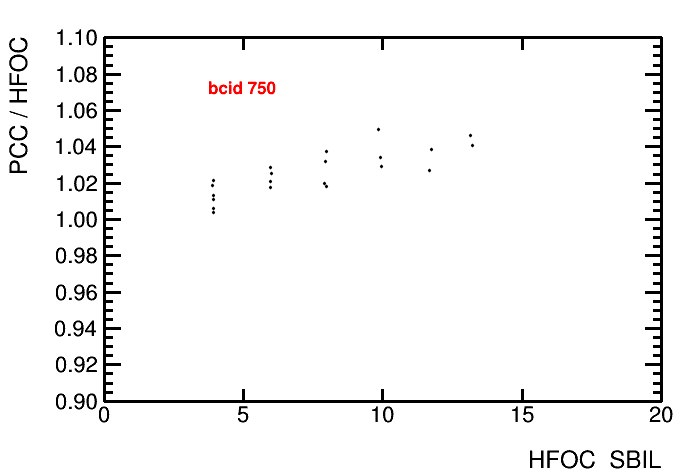
\includegraphics[width=0.47\linewidth]{plots/plot_det_linearity_perbx_pcc_7358_750_scatter.png}
    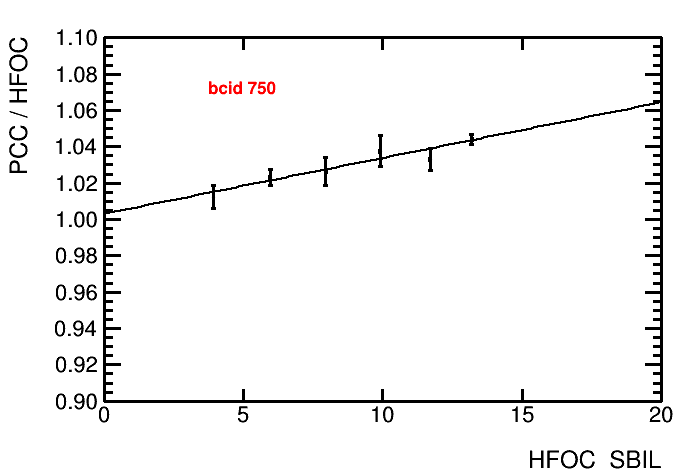
\includegraphics[width=0.47\linewidth]{plots/plot_det_linearity_perbx_pcc_7358_750_avg.png}
    \caption{
      PCC / HFOC  SBIL ratios as a function of HFOC SBIL for one bunch crossing in Fill 7358.
      The graphs illustrate the method for determining the average ratio at a given SBIL value as described in the text.
    \label{fig:sbilratiomethod}
    }
  \end{center}
\end{figure}

\clearpage
\begin{figure}[t]
  \begin{center}
    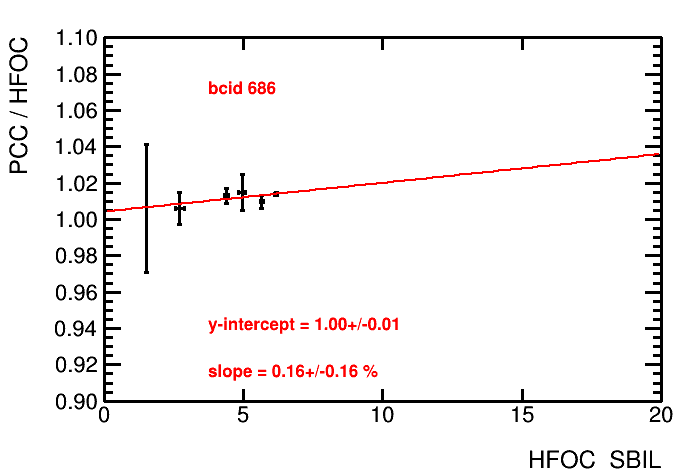
\includegraphics[width=0.47\linewidth]{plots/sbilratios_singles/plot_det_linearity_perbx_pcc_6847_686.png}
    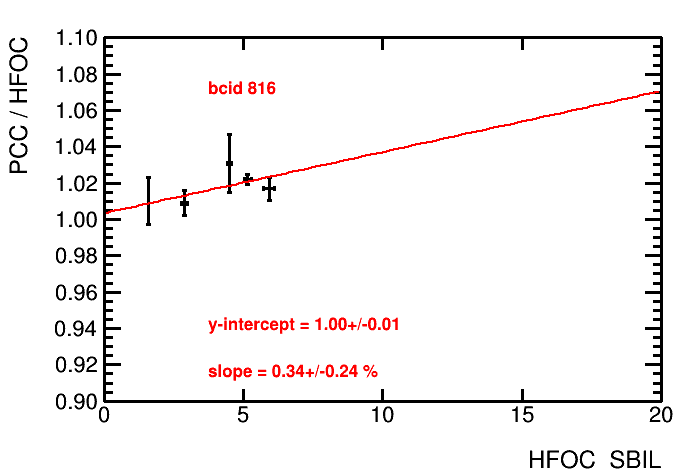
\includegraphics[width=0.47\linewidth]{plots/sbilratios_singles/plot_det_linearity_perbx_pcc_6847_816.png}
    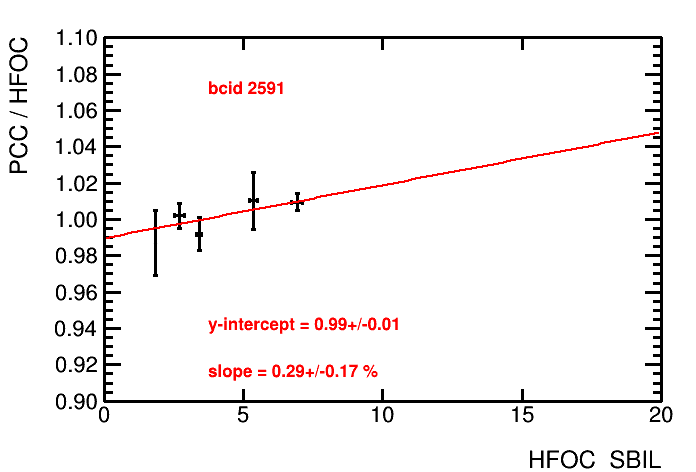
\includegraphics[width=0.47\linewidth]{plots/sbilratios_singles/plot_det_linearity_perbx_pcc_6847_2591.png}
    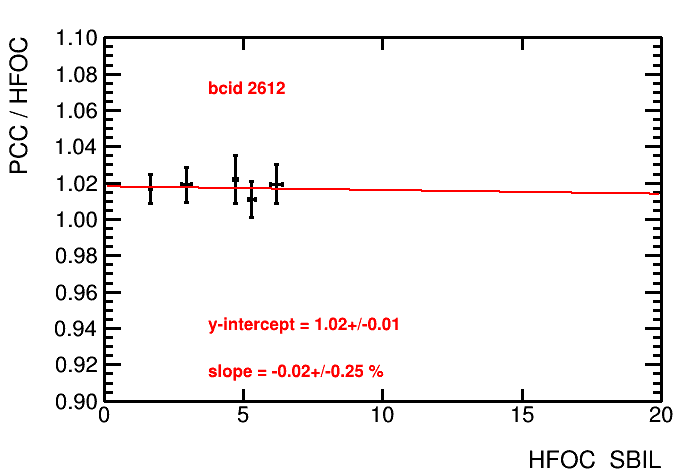
\includegraphics[width=0.47\linewidth]{plots/sbilratios_singles/plot_det_linearity_perbx_pcc_6847_2612.png}
    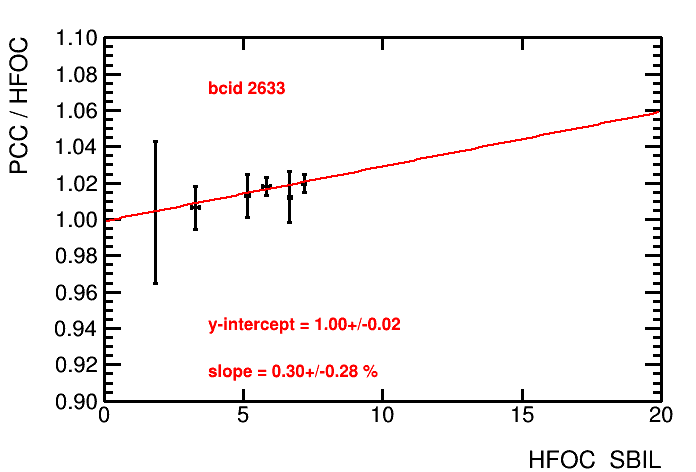
\includegraphics[width=0.47\linewidth]{plots/sbilratios_singles/plot_det_linearity_perbx_pcc_6847_2633.png}
    \caption{
      Ratio of PCC over HFOC single bunch instantenous luminosity (SBIL) as a function of SBIL for the 5 high statistics bunches in Fill 6847.
      The points and error bars are determined as described in the text.
    \label{fig:sbilratios6847}
    }
  \end{center}
\end{figure}

\clearpage
\begin{figure}[t]
  \begin{center}
    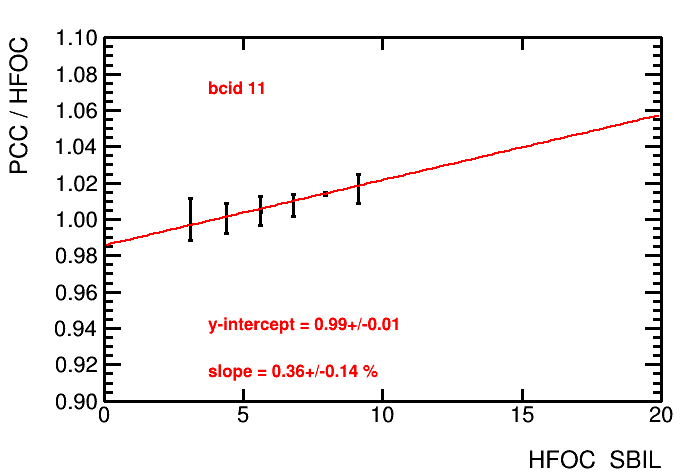
\includegraphics[width=0.47\linewidth]{plots/sbilratios_singles/plot_det_linearity_perbx_pcc_7358_11.png}
    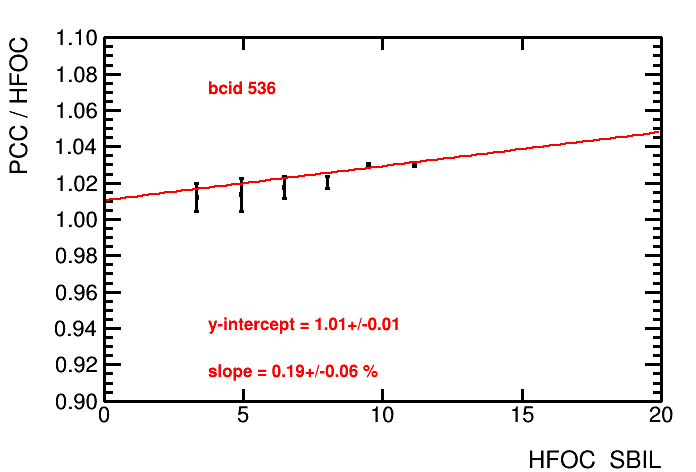
\includegraphics[width=0.47\linewidth]{plots/sbilratios_singles/plot_det_linearity_perbx_pcc_7358_536.png}
    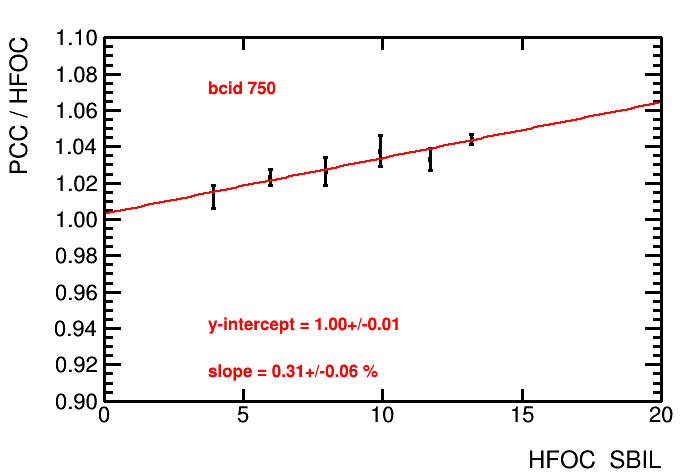
\includegraphics[width=0.47\linewidth]{plots/sbilratios_singles/plot_det_linearity_perbx_pcc_7358_750.png}
    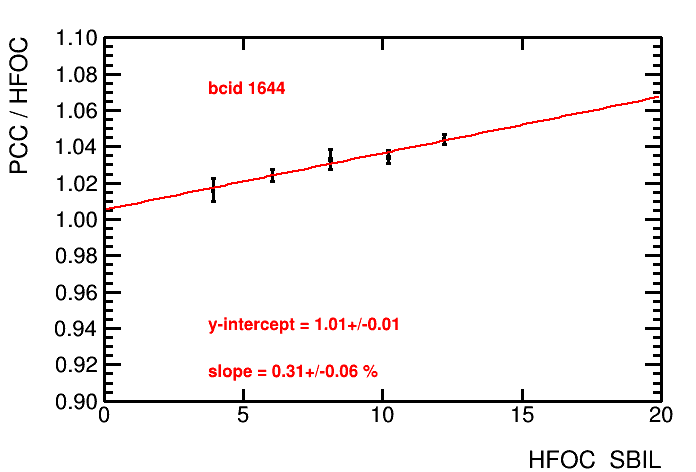
\includegraphics[width=0.47\linewidth]{plots/sbilratios_singles/plot_det_linearity_perbx_pcc_7358_1644.png}
    \caption{
      Ratio of PCC over HFOC single bunch instantenous luminosity (SBIL) as a function of SBIL for the 2 solo and 2 leading  bunches in Fill 7358.
      The points and error bars are determined as described in the text.
      \label{fig:sbilratios7358}
    }
  \end{center}
\end{figure}

\clearpage
\begin{figure}[t]
  \begin{center}
    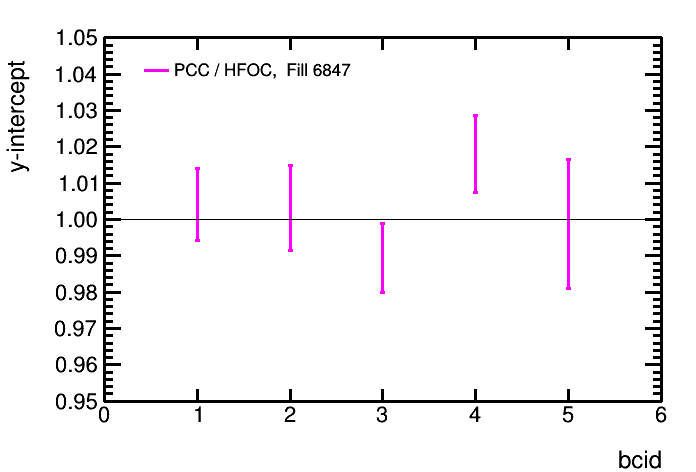
\includegraphics[width=0.47\linewidth]{plots/sbilratios_singles/plot_det_linearity_perbx_y0_6847.png}
    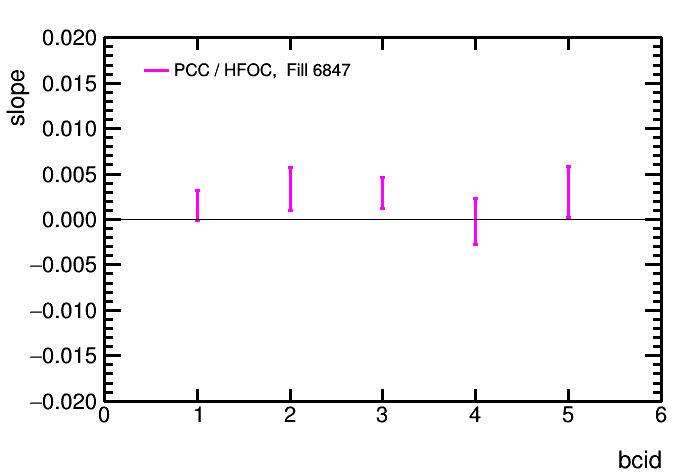
\includegraphics[width=0.47\linewidth]{plots/sbilratios_singles/plot_det_linearity_perbx_slope_6847.png}
    \caption{
      y-intercept (left) and slope (right) for the linear fits to the ratios of PCC/HFOC v.s. SBIL for the 5 high statistics bunches in Fill 6847.
      \label{fig:sbilratiosresults6847}
    }
  \end{center}
\end{figure}

\begin{figure}[t]
  \begin{center}
    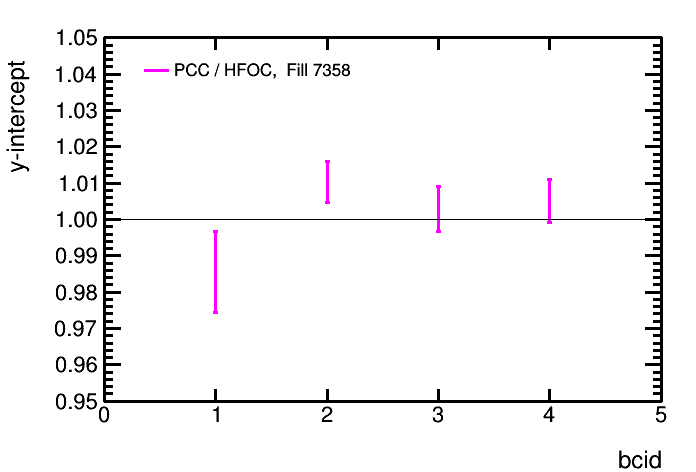
\includegraphics[width=0.47\linewidth]{plots/sbilratios_singles/plot_det_linearity_perbx_y0_7358.png}
    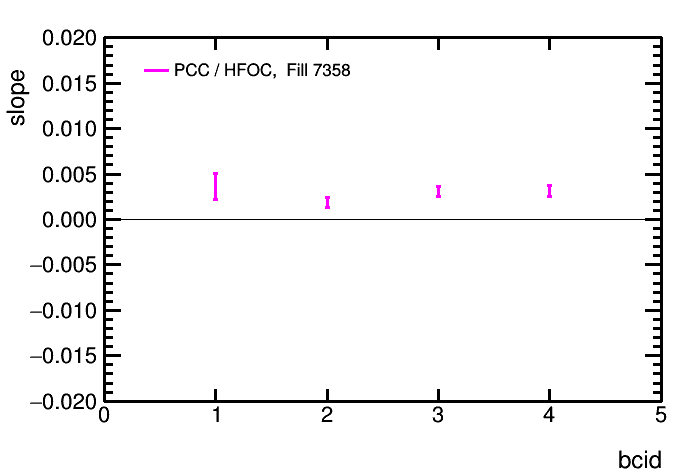
\includegraphics[width=0.47\linewidth]{plots/sbilratios_singles/plot_det_linearity_perbx_slope_7358.png}
    \caption{
      y-intercept (left) and slope (right) for the linear fits to the ratios of PCC/HFOC v.s. SBIL for the 2 solo and 2 leading  bunches in Fill 7358.
      \label{fig:sbilratiosresults7358}
    }
  \end{center}
\end{figure}


\clearpage
\begin{figure}[t]
  \begin{center}
    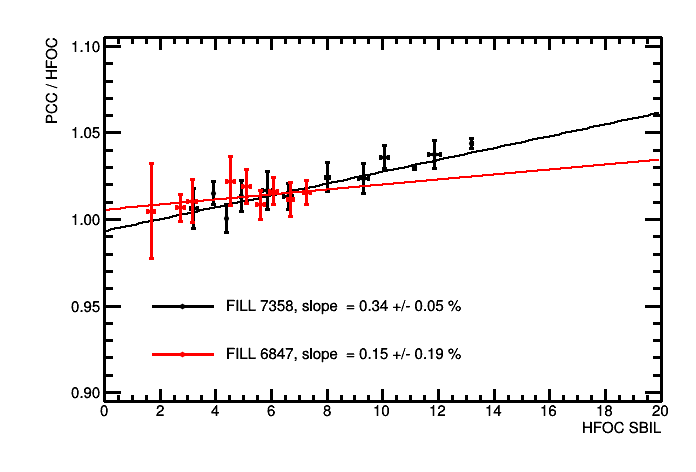
\includegraphics[width=0.7\linewidth]{plots/sbilratios_singles_combined/compareFills_graph_fillstogether.png}
    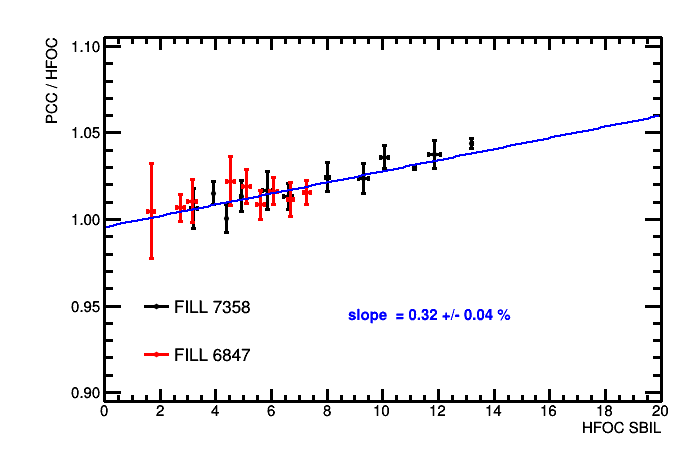
\includegraphics[width=0.7\linewidth]{plots/sbilratios_singles_combined/compareFills_graph_fillstogether_onefit.png}
    \caption{
      Comparison of the ratio of PCC / HFOC after combining all leading and solo bunches in fills 6847 and 7358.
      The data points and uncertainties are determined as described in the text.
      The fills are fit separately (top) and together (bottom).
      \label{fig:sbilratiosresultscombined}
    }
  \end{center}
\end{figure}


\clearpage
\begin{figure}[t]
  \begin{center}
    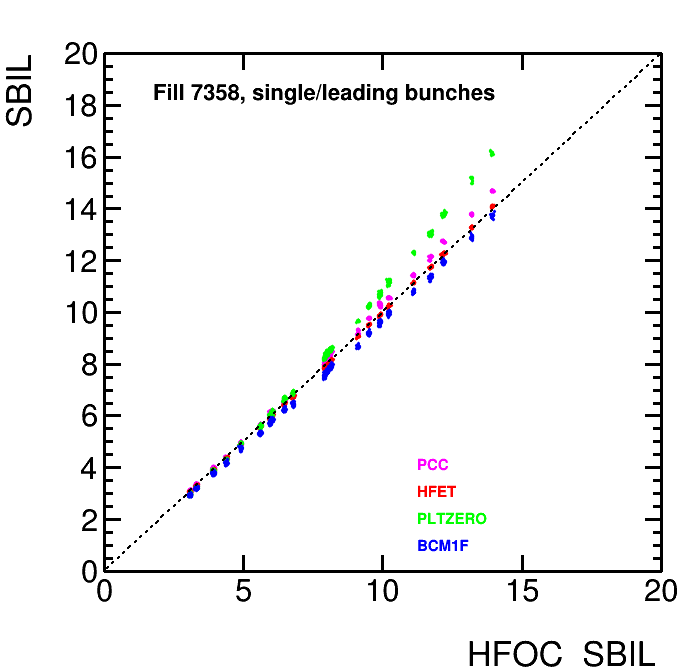
\includegraphics[width=0.47\linewidth]{plots/sbilratios_singles/plot_linearity_det_correlation.png}
    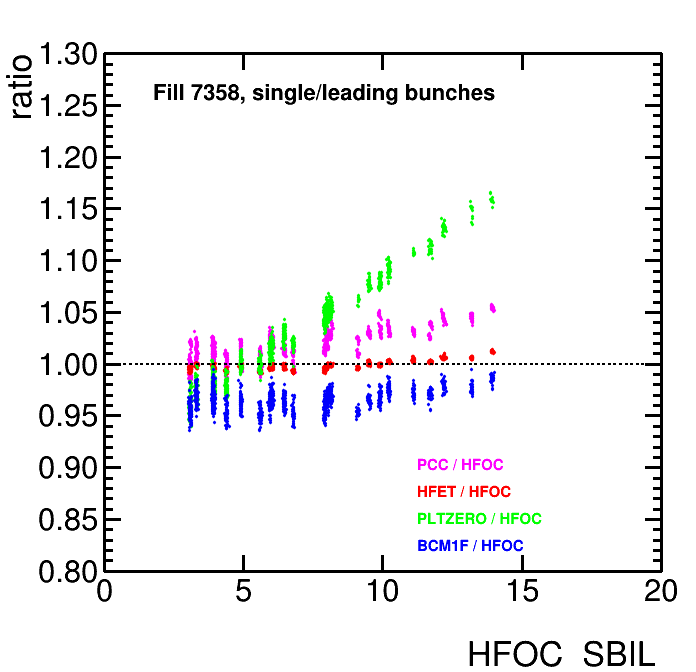
\includegraphics[width=0.47\linewidth]{plots/sbilratios_singles/plot_linearity_det_correlation_ratio.png}
    \caption{
      Correlations (left) and ratios (right) of the SBIL values between different luminometers in Fill 7358.
    \label{fig:sbilratios_dets}
    }
  \end{center}
\end{figure}
